\documentclass[class=report, crop=false, 12pt,a4paper]{standalone}
\usepackage{enumitem}
\usepackage{gensymb}
\usepackage{siunitx}
\usepackage{graphicx}
\usepackage[%
    labelfont=bf,
    format=hang,    
    format=plain,
    margin=0pt,
    width=0.8\textwidth,
]{caption}
\usepackage[list=true]{subcaption}
\sisetup{detect-all}
\begin{document}
\textbf{Insert solid structure lab report here}
\section{General link between properties and bonding}
\begin{figure}[h]
  \centering
  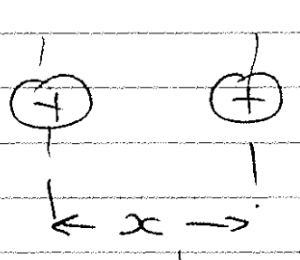
\includegraphics[width=0.3\textwidth]{../img/2atomsbonded}\caption{Two atoms bonded together at an equilibrium intermolecular distance $x$}
  \label{2atomsbonded}
\end{figure}
Consider two atoms bonded in a solid. Figure \ref{2atomsbonded} shows two atoms bonded together at a distance $x$ from each other - the equilibrium interatomic distance. There is a balance of two forces, the attractive "bond" and the repulsive; the nuclei are positively charged and thus repel. The distance $x$ will affect the fundamental properties e.g. optical properties.
\begin{figure}[h]
  \centering
  \subcaptionbox{Attractive \label{attractiveforce}}{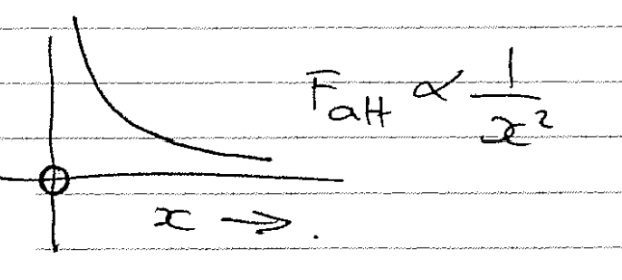
\includegraphics[width=0.30\textwidth]{../img/forcegraph1}}%
  \hfill
  \subcaptionbox{Repulsive \label{repulsiveforce}}{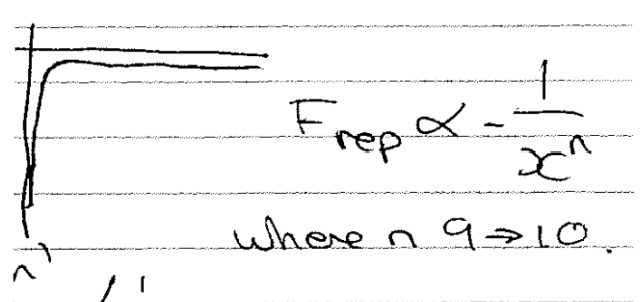
\includegraphics[width=0.30\textwidth]{../img/forcegraph2}}%
  \hfill
  \subcaptionbox{Total \label{totalforce}}{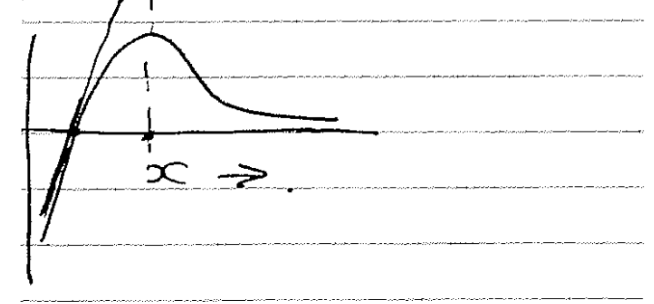
\includegraphics[width=0.30\textwidth]{../img/forcegraph3}}%
  \caption{Force graphs for two atoms bonded together.}
  \label{forcegraphs}
\end{figure}
The graphs shown in Figure \ref{forcegraphs} show the force of attraction (\ref{attractiveforce}), the force of repulsion (\ref{repulsiveforce}) and how the total force on the particle changes with $x$ (\ref{totalforce}). The attractive relationship (\ref{attractiveforce}) can be described as $F_{att} \propto \frac{1}{x^2}$. The repulsive relationship (\ref{repulsiveforce}) can be described as $F_{rep} \propto -\frac{1}{x^n}$ where n is between 9 and 10. Integrating (\ref{totalforce}) generates an energy response.
\subsection{Force-sum curve}
\begin{figure}[h]
  \centering
  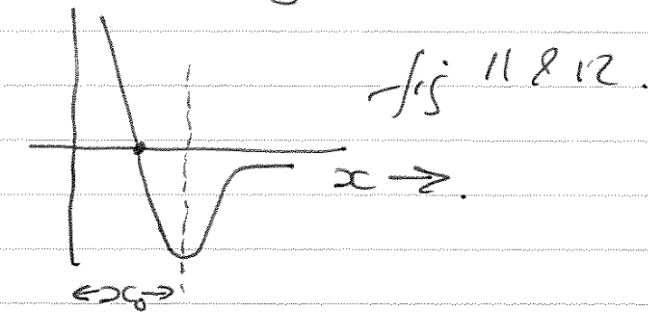
\includegraphics[width = 0.3\textwidth]{../img/energyresponse}
  \caption{Energy response as $x$ is varied}
  \label{fig:energyresponse}
\end{figure}
This crosses zero when $x = \textrm{interatomic distance}$ i.e. both forces are balanced - $x_0$. Displacement away from $x_0$ requires a net force to be applied. The peak of the force-sum curve can be related to the strength of the material. The slope of the curve when $x=x_0$ can be related to the stiffness of a material.
\subsection{Energy curve}
\begin{figure}[h]
  \centering
  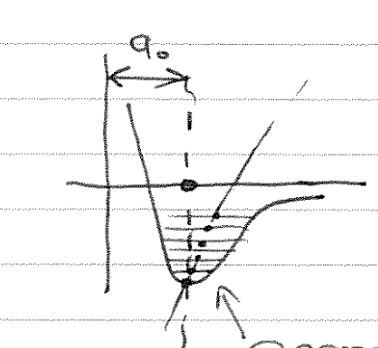
\includegraphics[width = 0.3\textwidth]{../img/energywell}
  \caption{The energy "well"}
  \label{fig:energycurve}
\end{figure}
The minimum of this curve occurs when $x=x_0$ - i.e. the material at equilibrium is at its lowest energy state. It is asymmetric about $x_0$. The depth of the well is related to how 'stable' a material is in the solid state. This related to the melting point of the substance (and its chemical reactivity). Also as heat (energy) input into such a system, the minimum moves to the right hand side (as the well fills up). This predicts that $a_0$ increases as heat is input i.e. materials expands on heating - expansion coefficient.
\section{Solidification of crystalline materials}
Regular solids (crystalline), that form at freezing point, start out via formation of a nuclei (small 'areas' (embryos) of crystalline material). These are nominally 200-300 atoms in diameter. They come about randomly, via collisions; this process is called nucleation. Once a nucleus of a given critical size has been created, crystals become stable at $R_{crit}$ and more atoms join, leading to the crystal growing. Anything smaller than $R_{crit}$, the crystal will remelt (because we are at the melting point as well as the freezing point). Because nuclei become stable, the heat (energy) they lose, needs to be removed, else solidification (into the surroundings) will stop (latent heat of solidification). This process is isothermal at the melting point and can be monitored using a cooling curve. Nucleating, being random, can occur anywhere and everywhere. This results is many crystals being formed and a polycrystalline solid being formed. This generates a characteristic cooling curve.
\begin{figure}[h]
  \centering
  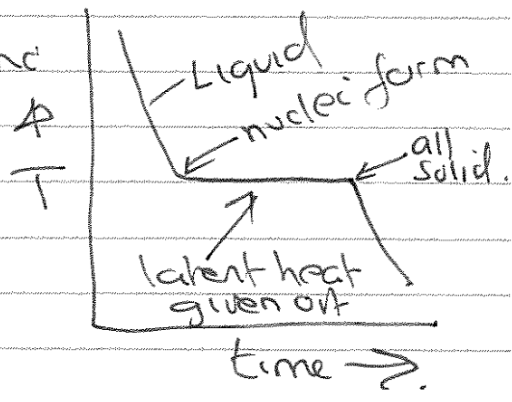
\includegraphics[width = 0.4\textwidth]{../img/coolingcurve}
  \caption{The characteristic cooling curve}
  \label{fig:coolingcurve}
\end{figure}[h]
\subsection{Practical casting}
\begin{figure}
  \centering
  \subcaptionbox{Initial nucleation \label{fig:practicalcasting1}}{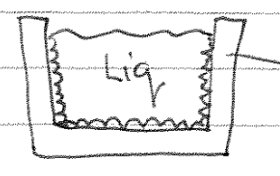
\includegraphics[width=0.30\textwidth]{../img/practicalcasting1}}%
  \hfill
  \subcaptionbox{Growth of nuclei \label{fig:practicalcasting2}}{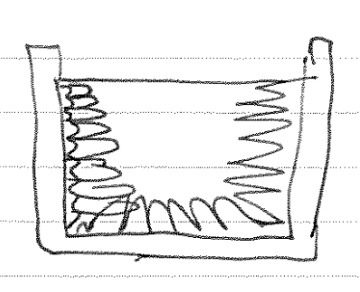
\includegraphics[width=0.30\textwidth]{../img/practicalcasting2}}%
  \hfill
  \subcaptionbox{Columna \label{fig:practicalcasting3}}{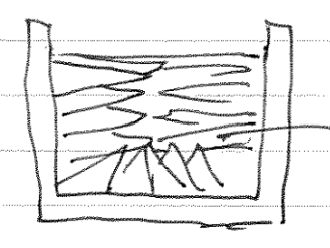
\includegraphics[width=0.30\textwidth]{../img/practicalcasting3}}%
  \caption{The nucleation process}
  \label{fig:nucleationprocess}
\end{figure}
Many nuclei are formed but on walls of the mould (\ref{fig:practicalcasting1}). Subsequently crystals grow from the nuclei into the centre of the mould (\ref{fig:practicalcasting2}) - long and thin "columna" crystals (grains) (\ref{fig:practicalcasting3}). Nuclei are formed by random means i.e. we get lots of crystals; there is no orientation relationship between each nucleus. Hence, misorientated crystals cannot join perfectly. This results in a polycrystalline solid grain structure aka a microstructure \si{\micro\meter} - \si{\milli\meter} in dimension. This strongly influences properties and can easily be altered via manufacturing processing. e.g. columna grains - typical of an 'open' casting are not ideal - better mechanical properties can be achieved if grains are polygonal and approximately equal sized in 3 orthogonal directions: equiaxed crystals (\ref{fig:equiaxed}). This can be achieved via rapid cooling.
\begin{figure}[h]
  \centering
  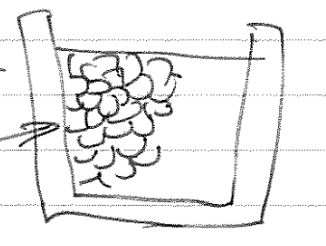
\includegraphics[width = 0.4\textwidth]{../img/equiaxed}
  \caption{Equiaxed crystal structure}
  \label{fig:equiaxed}
\end{figure}
When grains eventually touch they cant join perfectly - so they create an area of 'disorder' - i.e. high energy (thermodynamically) - not fully crystalline. This is the grain boundary. Due to higher free energy, grain boundaries are more likely to host chemical reactions or processes that decrease free energy. e.g. oxidation/corrosion. They are also significant in determining mechanical properties. 

During cooling if a material is very pure and/or the mould is extremely pure/clean, it is possible to avoid nucleation and hence cool to below freezing point. This is called undercooling. n.b. extreme undercooling - called supercooling - results in no crystalline structures forming: an amorphous solid (supercooled, high viscosity liquids)
\begin{figure}[h]
  \centering
  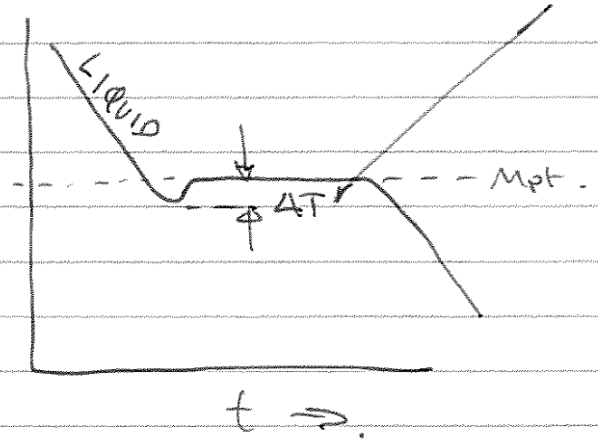
\includegraphics[width = 0.4\textwidth]{../img/supercooling}
\end{figure}
Once nucleation begins, the crystallisation process wil rapidly occur. Undercooling can be generated by rapid cooling of a mould. This is more common in materials that find it difficult to crystallize e.g. long chain thermopolymers and $SiO_2$ ceramics. Undercooling, therefore, occurs more easily in complex crystal structures - in a metal, a $\Delta T$ is almost impossible to observe. It is possible to see in ultra pure metals and/or if cast into a very clean mould. Why? $\Delta T$ is related to the time it takes to create stable nuclei - i.e. reach $R_{crit}$.
\begin{figure}[h]
  \centering
  \subcaptionbox{Sphere \label{fig:rcritfull}}{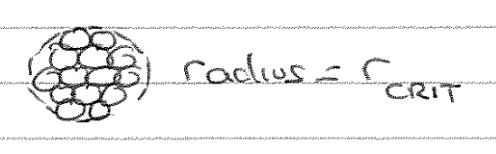
\includegraphics[width=0.45\textwidth]{../img/rcritfull}}%
  \hfill
  \subcaptionbox{Hemisphere \label{fig:rcrithalf}}{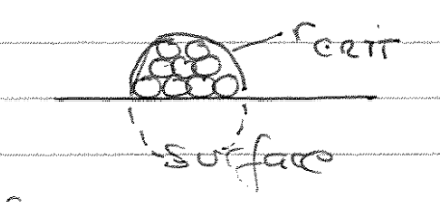
\includegraphics[width=0.45\textwidth]{../img/rcrithalf}}%
  \caption{Different sorts of nuclei formation}
\end{figure}
$R_{crit}$ is a radius - achievable either by creating a sphere of atoms or a hemisphere of atoms. Thus, if a surface is available it can reduce the requirement for the number of atoms to create a $R_{crit}$ (is a random process - so more chance of happening) i.e. surfaces help nucleation and act as sites for nucleation. There are two types of nucleation that we can define: self nucleation (homogeneous nucleation) and heterogeneous (nucleation on something). The nucleation type affects microstructure. 
\begin{figure}[h]
  \centering
  \subcaptionbox{Heterogeneous nucleation X1}{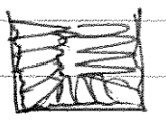
\includegraphics[width=0.45\textwidth]{../img/heteronucleation}}%
  \hfill
  \subcaptionbox{Homogeneous nucleation\\ (or hetero if impure) X1A}{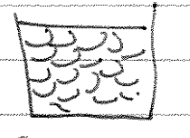
\includegraphics[width=0.45\textwidth]{../img/homonucleation}}%
\end{figure}
Commercially done by adding innoculants e.g. Ti02 Si02 powder. Also known as seeding. 

In many crystalline solids, the process of solidification goes through a dendritic stage. dendrite - from greek for tree - dendra - 3D crystal
\begin{figure}[h]
  \centering
  \subcaptionbox{}{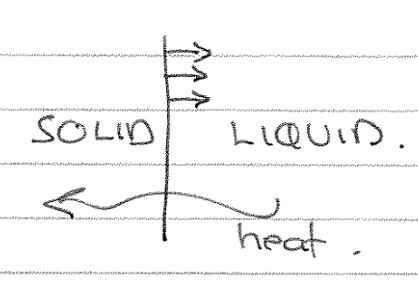
\includegraphics[width=0.45\textwidth]{../img/dendriticgrowth4}}%
  \hfill
  \subcaptionbox{}{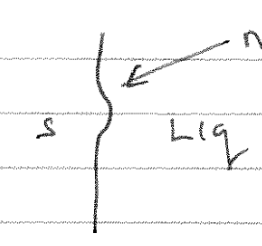
\includegraphics[width=0.45\textwidth]{../img/dendriticgrowth3}}%
\end{figure}
Dendrites emerge from nominally stable S-L growth fronts and would normally melt back - but under certain circumstances any protruberance becomes stable
\begin{figure}
  \centering
  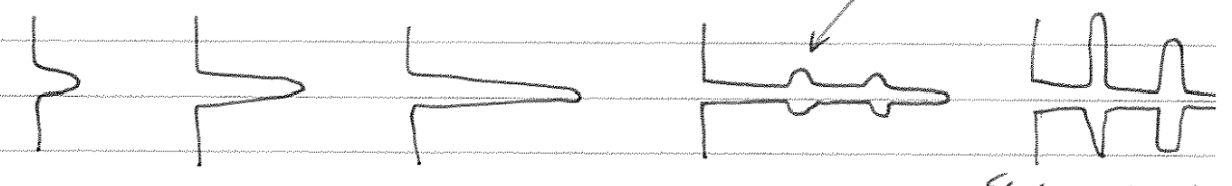
\includegraphics[width = \textwidth]{../img/dendriticgrowth2}
\end{figure}
e.g. see constitutional supercooling. more likely in impure substances
\begin{figure}[h!]
  \centering
  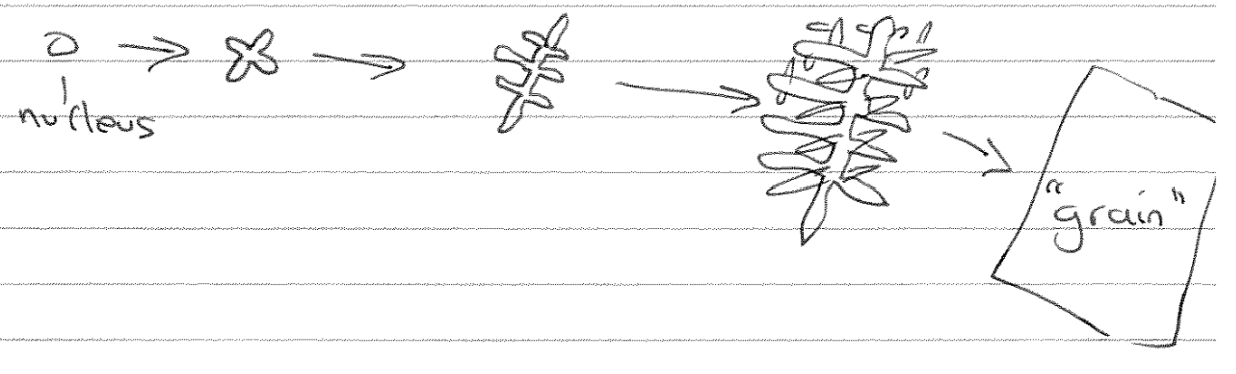
\includegraphics[width = \textwidth]{../img/dendriticgrowth}
\end{figure}
normally a growing dendrite will fill space gradually and become a single crystal and in disappear. 

Two occasions when dendrites appear in the microstructure: coring - variation in the composition of a dendrite as it grows revealing the stages of dendritic growth e.g. as colour changes. gradual change in composition - microsegregation. every grain will be cored, can compromise corrosion resistance and mechanical properties. or if the space in between the dendrite arms are filled with another substance (phase see X6 and X7). 

in casting technology, coring is regarded as a defect but there are others, principally porosity - holes in the microstructure. they can seriously degreade/affect mechanical properties. act as stress concentrators. 
\end{document}